\documentclass[11pt,a4paper]{article}
\usepackage{amsmath}
\usepackage{amssymb}
\usepackage{fullpage}
\usepackage{graphicx}
\usepackage[colorlinks=true, linkcolor=blue]{hyperref}

\newcommand{\argmin}{\operatornamewithlimits{arg\,min}}
\renewcommand{\arraystretch}{1.15} % line spacing in tabular

\begin{document}
\title{Improving Image Understanding with Concept Graph}
\author{Libo Yin\\The Australian National University}
\maketitle
\section{The Original HEX Model}
\subsection{Structure}

The original HEX model \cite{deng2014large} is an extension of the baseline flat multiclass classification model. There are two types of multiclass classification: exclusive, where the classifier predicts exactly one out of all possible states to be true; and independent, where each state is predicted true or false independently. HEX finds a balance between these two ends of the spectrum. It models the Hierarchical and EXclusive relationship within the concept space of dataset, extended by their hypernyms, with a semantic graphical model. Each node in the HEX graph corresponds to a concept in the extended concept space being true or false. States of neighbouring nodes are constrained in that if $a$ is a hypernym of $b$, then is not allowed that $a=0,\ b=1$; and if $a$ and $b$ are exclusive, then they cannot both be true. HEX model classifies an image into a joint assignment of the states of nodes, corresponding to a hierarchy in the graphical model, that satisfies the above semantic consistency. A simple HEX graph is shown in \hyperref[fig:naive]{figure~\ref{fig:naive}}.
\begin{figure}[htbp]
\centering
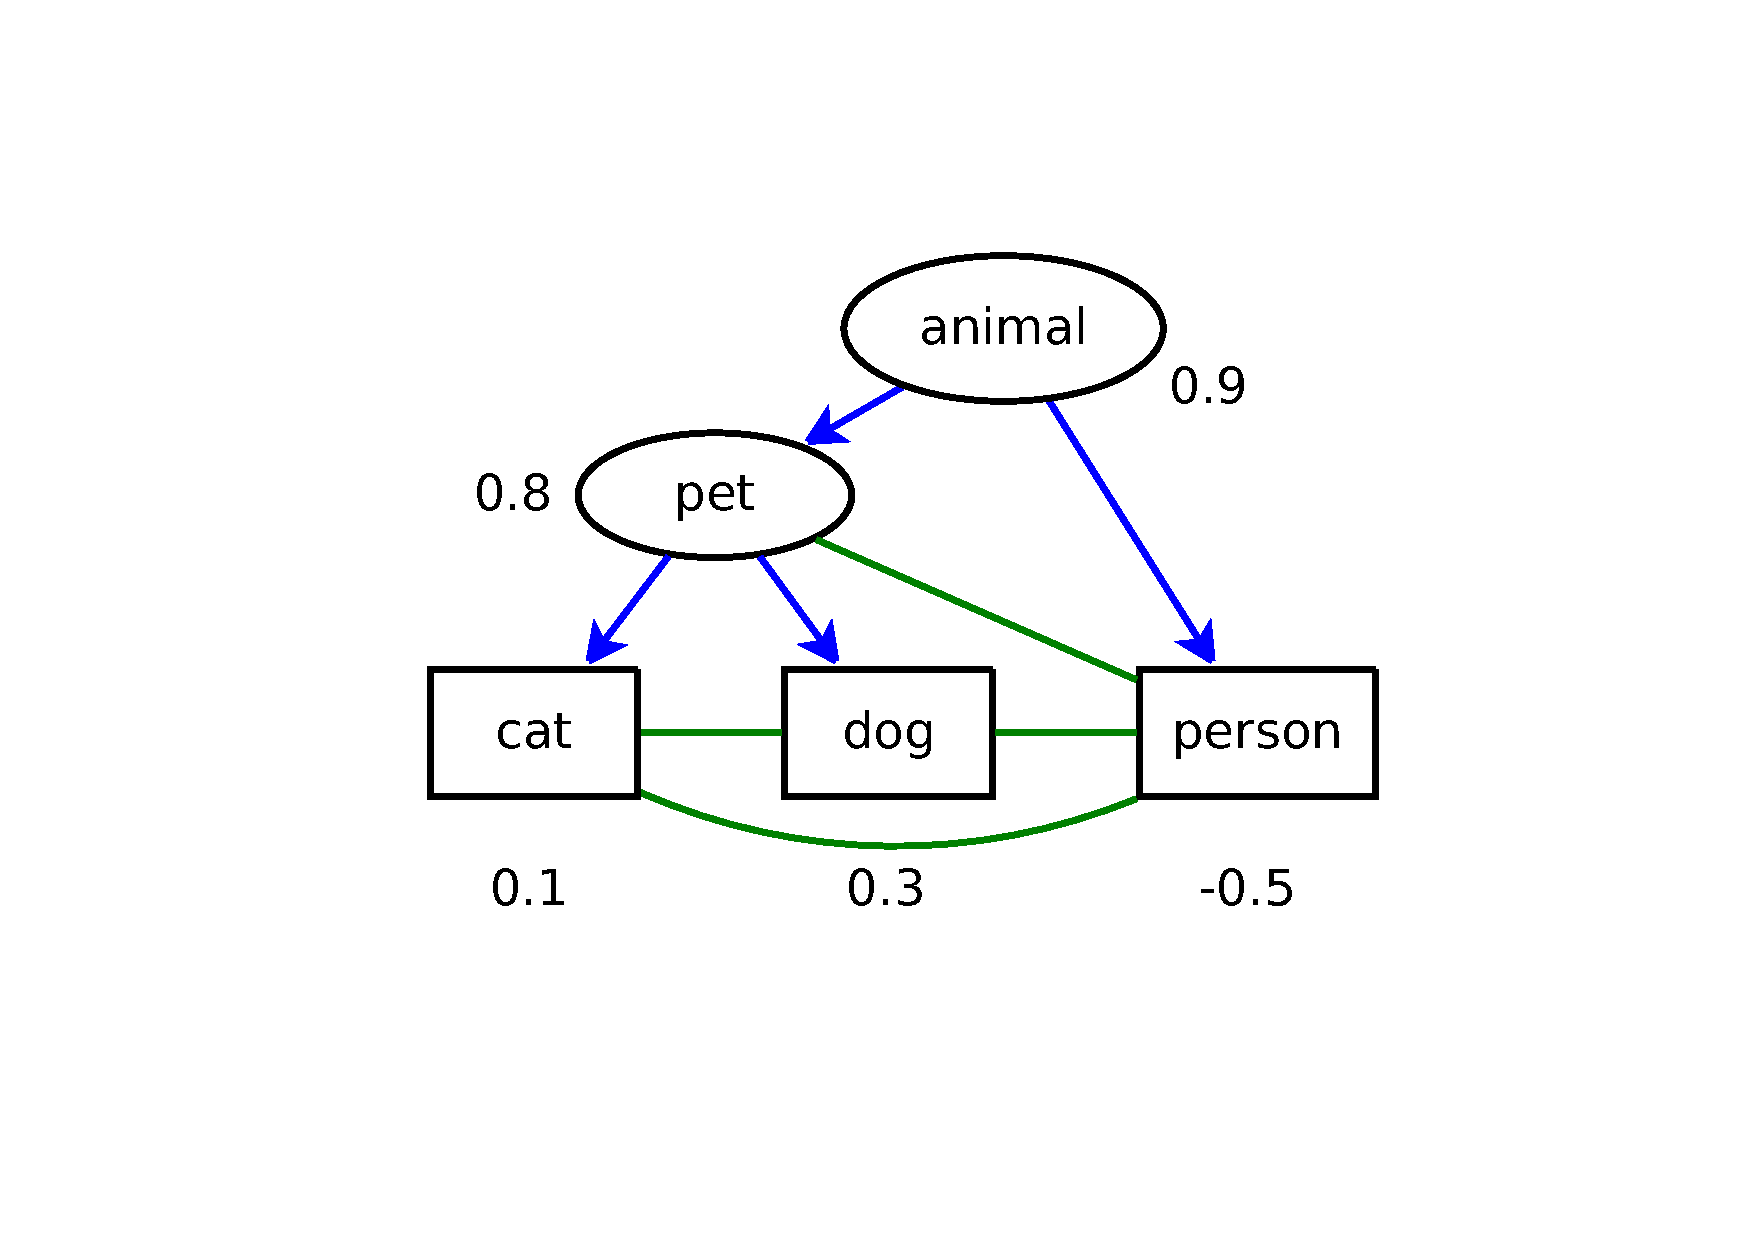
\includegraphics[scale=0.5]{naive.pdf}
\caption{A simple HEX graph with three nodes in the original concept space (in rectangles) and their hypernyms (in ellipsoids). Directed edges denote semantical subsumption: $(a\rightarrow b)$ if $a$ is a hypernym of $b$ according to WordNet; and undirected edges denote exclusion. Since exclusive relationship is not covered by WordNet, the exclusive subgraph is initialized greedily: two concepts are exclusive unless they share a common descendant in the hierarchical subgraph. Note that the hierarchical subgraph is in general a DAG rather than a tree; and it is not necessarily the case that all concepts in the original concept space are bottom-level nodes in the hierarchical subgraph. Values beside each nodes are to be used in \hyperref[tab:naive]{table~\ref{tab:naive}}.}
\label{fig:naive}
\end{figure}

Denoting the set of vertices by $V$, the set of hierarchical edges by $E_h$, and the set of exclusive edges by $E_e$, the joint assignment $y\in\{0,1\}^V$ can be defined as a conditional random field:
\begin{equation}
\tilde{p}(y|x)=\prod_{i\in V}\exp\{f_i(x;w)I[y_i=1]\}I[y\text{ legal}]
\label{eqn:naive}
\end{equation}

where unary input $f_i(x;w)$ is the confidence on concept $i$, predicted by an arbitrary underlying classifier\footnote{According to \cite{deng2014large}. It shall be explained in \hyperref[sec:observ]{section~\ref{sec:observ}} that the choice of underlying unary classifier is actually not arbitrary.}. Local semantic constraints on hierarchical and exclusive edges is formalised by:
\begin{equation}
I[y\text{ legal}]=\prod_{(v_i,v_j)\in E_h}I[(y_i,y_j)\neq(0,1)]\prod_{(v_i,v_j)\in E_e}I[(y_i,y_j)\neq(1,1)]
\label{eqn:legal}
\end{equation}

Thanks to these semantic constraints, the state space of a HEX graph, i.e.\ the set of all legal joint assignments, is significantly smaller than the state space of independent multiclass classification on the same concept space. For example, with local confidence given beside each node in \hyperref[fig:naive]{figure~\ref{fig:naive}}, the valid assignments of the HEX graph and their respective potentials are listed as follows:

\begin{table}[htbp]
\centering
\begin{tabular}{r|l}
assignment & $\tilde{p}(y|x)$\\
\hline
$\varnothing$ & $\exp(0)$\\
\{animal\} & $\exp(0.9)$\\
\{animal, pet\} & $\exp(0.9+0.8)$\\
\{animal, person\} & $\exp(0.9-0.5)$\\
\{animal, pet, cat\} & $\exp(0.9+0.8+0.1)$\\
\{animal, pet, dog\} & $\exp(0.9+0.8+0.5)$\\
\{animal, pet, dog, Husky\} & $\exp(0.9+0.8+0.5-0.1)$\\
\{animal, pet, dog, Labrador\} & $\exp(0.9+0.8+0.5+0.3)$
\end{tabular}
\caption{The extended state space, i.e.\ all valid assignments of the HEX graph in \hyperref[fig:naive]{figure~\ref{fig:naive}}, and their respective potentials. In this example, the most likely joint assignment is \{animal, pet, dog, Labrador\}. The softmax baseline classifier, in the language of HEX, classifies to the original state space: \{animal, pet, cat\}, \{animal, pet, dog\}, \{animal, pet, dog, Husky\}, \{animal, pet, dog, Labrador\}, and \{animal, person\}.}
\label{tab:naive}
\end{table}

Finally, an important assumption of \cite{deng2014large} is that mechanical Turks tend to label an image to more abstract concepts. For example, an image of a yellow Labrador is more likely to be labelled to ``dog'' than ``Labrador''. Such behaviour is modelled by randomly relabelling images to their immediate parents. As will be shown in \hyperref[sec:exp1]{section~\ref{sec:exp1}}, the higher the relabelling rate is, the larger is the advantage of the HEX model compared to the softmax baseline.

\subsection{Observations}
\label{sec:observ}

Note that a valid assignment does not have to have an active node in the original concept space. (Actually, it does not have to have an active node at all, as $\varnothing$ is a valid joint assignment according to \hyperref[eqn:legal]{(\ref{eqn:legal})}.) This allows an image to be classified to a joint assignment in which all active concepts are abstract. For example, in \hyperref[fig:naive]{figure~\ref{fig:naive}}, \{$\varnothing$\}, \{animal\}, or \{animal, pet\}. This is by no doubt a desirable feature for deployment. However, since all images are labelled in the original concept space, classifying to the extended concept space makes performance evaluation troublesome. While this issue is not addressed in \cite{deng2014large}, the evaluation strategy used for this work will be discussed in \hyperref[sec:exp1]{section~\ref{sec:exp1}}.

Also note that in \hyperref[tab:naive]{table~\ref{tab:naive}}, the competition between assignment \{animal, pet, dog, Husky\} and \{animal, pet, dog, Labrador\} depends entirely on the confidence of node ``Husky'' and ``Labrador''. However, to discriminate between \{animal, pet, dog, Husky\} and \{animal, person\} requires examining the confidence along different paths. From this example it is clear that, in the testing stage, confidence is passed down the hierarchy from more abstract concepts to more concrete ones. The other side of the same coin is that, during the training stage of the underlying unary classifier, a node corresponding to abstract concepts receive all training data of its children. This can be seen as confidence being passed up in the hierarchy, from more concrete concepts to more abstract ones. Such bidirectional propagation of confidence explains the advantage of the HEX model under the realistic labelling assumption. Note that the exclusive subgraph does not take part in the propagation of confidence.

The third observation is a combined consequence of the greedy exclusion setup, as discussed under \hyperref[tab:naive]{table~\ref{tab:naive}}, and the greedy nature of the potential function \hyperref[eqn:naive]{(\ref{eqn:naive})}. The prerequisite for the original HEX model is that the decision boundary of $f_i(x;w)$ is zero for all $i$: A unary prediction above zero gives support to a node being active (true), whereas a unary prediction below zero gives support to that node being inactive (false). In \cite{deng2014large} this is not a problem, as a convolutional neural network \cite{krizhevsky2012imagenet} is used as the underlying unary classifier; and that the a neural network can learn its decision boundary form training data. However, if a probabilistic classifier is used, in which case $f_i(x;w)\in[0,1]$ and the decision boudary is 0.5, then it is guaranteed that a bottom-level node will be activated (see \hyperref[sec:fail]{appendix~\ref{sec:fail}} for proof). This means that the effective state space size of the HEX graph is reduced to the number of bottom-level nodes, which is no larger than the original state space size. This defeats the purpose of HEX, although a smaller state space means faster inference and higher accuracy.

Finally, listed below are two less important observations:
\begin{enumerate}
\item There are no learnable variables in this CRF. In other words, all learning is performed in the underlying unary classifier.
\item Mathematically, CRF requires $\forall y:\tilde{p}(y|x)>0$. However, computationally, assigning zero to $\tilde{p}(y|x)$ can be interpreted as assigning an infinitesimal value. Therefore, the above definition is computationally a legitimate CRF.
\end{enumerate}

\subsection{Problems}
\label{sec:problem}

\begin{figure}[htbp]
\centering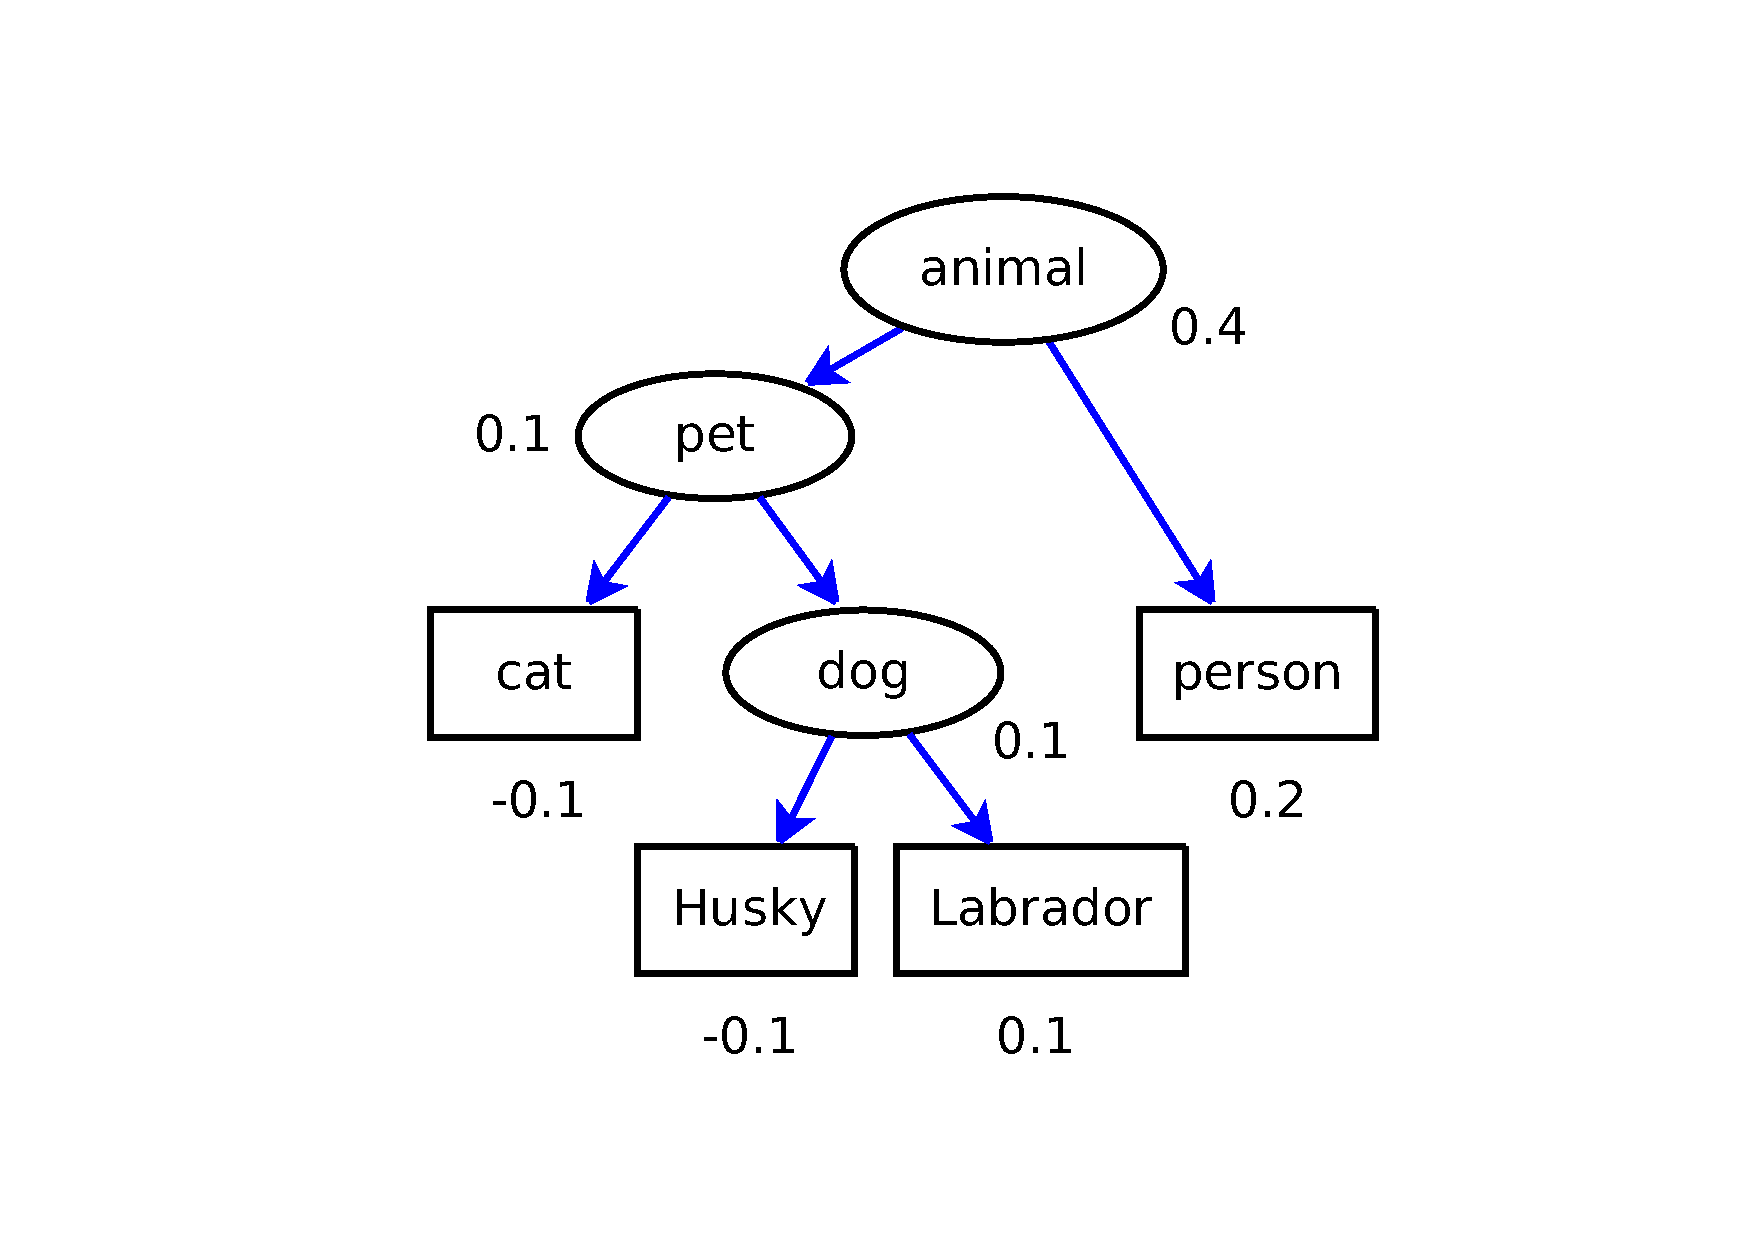
\includegraphics[scale=0.5]{depth.pdf}
\caption{Where an assignment with more active nodes of lower confidence wins over an assignment with fewer active nodes of higher confidence. Exclusive edges are not drawn, as they do not carry further information once the state space has been calculated.}
\label{fig:depth}
\end{figure}

Consider the situation illustrated in \hyperref[fig:depth]{figure~\ref{fig:depth}}. Following the same logic as \hyperref[tab:naive]{table~\ref{tab:naive}}, the original HEX model predicts \{animal, pet, dog, Labrador\}. However, this is a result of more active nodes rather than active nodes of higher confidence. Intuitively, \{animal, person\} seems a more reasonable prediction. In addition, the two aforementioned assignments are only separated by 0.1 in log unnormalised potential. It will be desirable if the model can make a prediction that is further from the decision boundary by taking into account the confidence of other nodes, especially those with unary predictions far from the decision boundary.

The second problem is a combined consequence of the realistic labelling assumption and using CNN as the underlying unary classifier. When the relabelling rate is high, most images are relabelled to their immediate parents. This means that for each concept $X$, most instances of $X$ are correctly labelled to all its ancestors, but incorrectly labelled ``NOT $X$''. This create a highly unbalanced and internally inconsistent dataset. In such case, because CNN is trained as an independent multiclass classifier, the unary predictions will highly likely be ``NOT $X$'' for images of $X$. (This hypothesis will be confirmed in \hyperref[sec:exp1]{section~\ref{sec:exp1}}.) The original HEX model does not cope with such situation, as the potential function \hyperref[eqn:naive]{(\ref{eqn:naive})} deactivates a bottom-level node as long as its unary confidence is below the decision boundary.

\clearpage
\section{Reimplementation}
\subsection{Dataset}
\label{sec:data}

The original HEX model is reimplemented as the baseline of this work. While \cite{deng2014large} used ILSVRC 2012 dataset for its rich structure in the label space, this work employs PASCAL VOC 2012 \cite{pascal-voc-2012} for its simplicity. The complete hierarchical subgraph of HEX is shown in \hyperref[fig:hex]{figure~\ref{fig:hex}}. Note that the two datasets are designed for different tasks: ILSVRC is an exclusive multiclass classification problem, whereas PASCAL is an independent multiclass classification problem. To adapt to ILSVRC task 1, the train+val dataset of PASCAL is filtered through the following criteria:
\begin{enumerate}
\item If there is only one annotated object in the image, the image is labelled to that object.
\item If the largest annotated object in the image is more than twice as large as the second largest one, the image is labelled to its dominating object.
\end{enumerate}

Another major difference between ImageNet and PASCAL is that the former one is a balanced dataset, while the latter is highly unbalanced. For example, after filtering, there are 5,324 images labelled as ``person'', whereas the second most frequent label ``dog'' has only 817 instances. To rebalance the dataset, 950 images of ``person'' are subsampled from the filtered dataset.  After preprocessing, the dataset contains 8,473 images in total. These images are then split 3:1:1 into train/validation/test set. The distribution of images across labels is illustrated in \hyperref[fig:distro]{figure~\ref{fig:distro}}.
\begin{figure}[htbp]
\centering
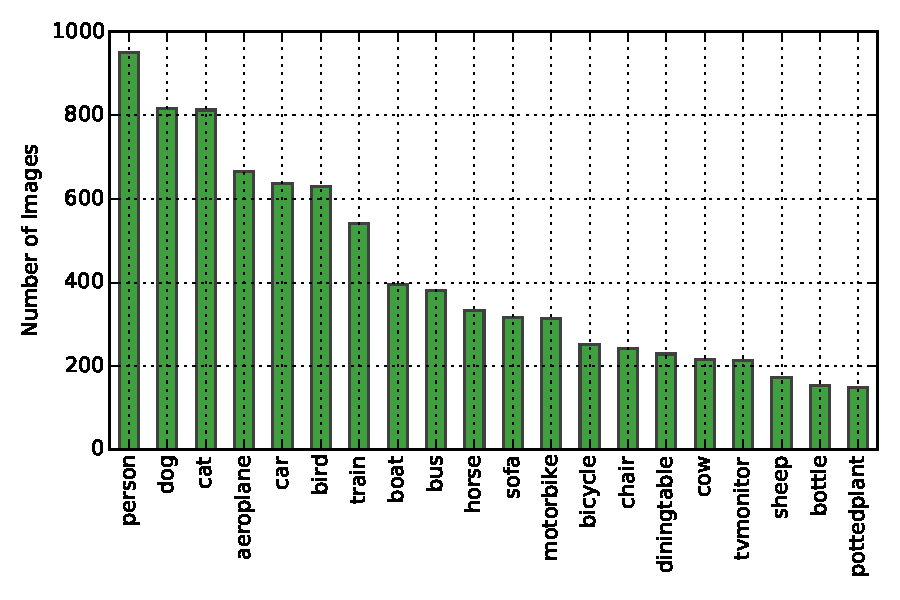
\includegraphics[scale=0.8]{distro.pdf}
\caption{Distribution of images according to labels, after preprocessing.}
\label{fig:distro}
\end{figure}
\begin{figure}[p]
\centering
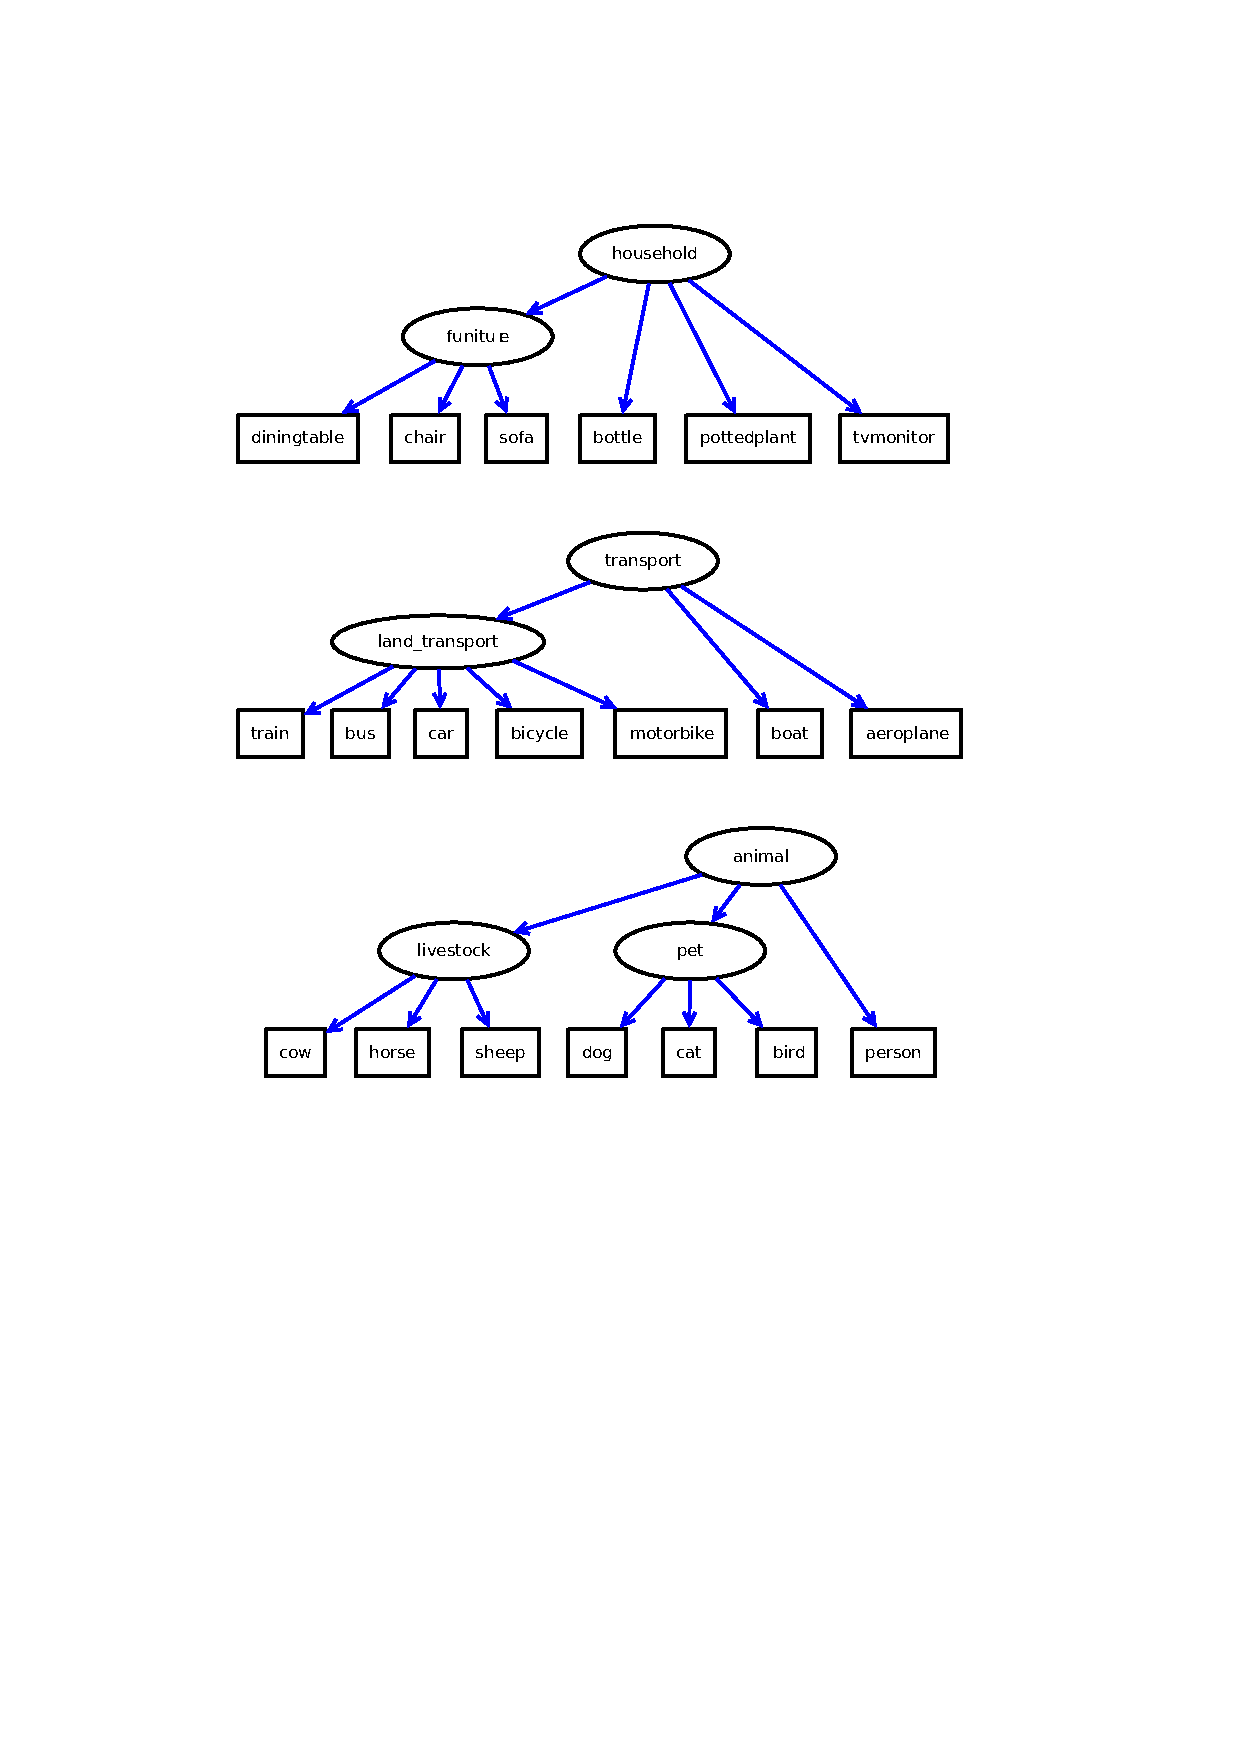
\includegraphics[scale=1]{full.pdf}
\caption{The PASCAL dataset has 20 concepts, as shown in rectangles. In this work, these concepts are extended by 7 of their hypernyms, creating a forest of three trees with 27 nodes and 24 hierarchical edges. Exclusive edges are not drawn since they can be implied by the hierarchical subgraph. The state space of this HEX graph has size 28. In comparison, the HEX graph in \cite{deng2014large} contains 1000 nodes corresponding to the original concept space, and 820 nodes corresponding to their hypernyms. Note that there is no hierarchical relationship within the original concept space.}
\label{fig:hex}
\end{figure}

\clearpage
\subsection{Algorithms}

For consistency with \cite{deng2014large}, the underlying unary classifier is based on \cite{krizhevsky2012imagenet} instead of the current state-of-the-art \cite{simonyan2014very}. The CNN, originally trained on ImageNet, is fine-tuned as an independent multiclass classifier on PASCAL, where each image is projected to a 27-dimensional vector. Note that since the original HEX model has no learning part, it was built as a layer into the CNN, achieving end-to-end learning. In this work, CNN and CRF are implemented separately, such that multiple variants of the HEX model can be tested with the same CNN as underlying unary classifier. For details of CNN setup, refer to \hyperref[sec:setup]{appendix~\ref{sec:setup}}.

A simpler concept space also lead to the change of inference algorithm. In \cite{deng2014large}, inference is performed by MAP loopy belief propagation on the HEX graph, where the local state space of each clique is constrained by semantic restrictions. In this work, due to the small concept space of dataset, the inference is performed by calculating the potential function directly for each state in the global state space.

Finally, to guarantee that the benefit of the HEX model is consistent regardless of the underlying unary classifier, different variants of the HEX model are also paired with SVM as the underlying unary classifier. An array of 27 SVMs is trained, each corresponding to a node in the HEX graph. The SVM array accepts the output of the last-but-one layer of \cite{krizhevsky2012imagenet} as input, assuming that 4,096 neurons provide sufficiently diverse and accurate feature responses \emph{without} fine-tuning on the PASCAL dataset. The SVM array predicts either distance to decision boundaries (corresponding to raw CNN output), or the probability of each concept being activated (corresponding to CNN output with sigmoid transformation). For the detail of SVM setup, refer to \hyperref[sec:setup]{appendix~\ref{sec:setup}}.

\subsection{Experiments}
\label{sec:exp1}

In this work, accuracy is tested both in the extended state space and in the original one, by limiting the legal state space to assignments with an active bottom-level node in the hierarchical subgraph. Note that this is only valid for datasets where all concepts in the original concept space are bottom-level nodes in the HEX graph.

The empirical test result of \cite{deng2014large} and reimplementation are compared in \hyperref[tab:original]{table~\ref{tab:original}}. Note that due to the size of PASCAL dataset, relabelling rate of 95\% is not attempted in this work. Observations on the result are listed as follows:
\begin{enumerate}
\item Regardless of implementation and inference algorithm, the accuracy drops as the relabelling rate grows.
\item With extended state space, independent multiclass classification by itself tend to have the lowest accuracy. However, with the HEX model as a noise filter, classification information can be recovered to a similar level as the softmax baseline.
\item In \cite{deng2014large}, the original HEX model managed to beat the softmax baseline under all relabelling rates. However, with the reimplemented system and the extended state space, the accuracy of HEX falls below the softmax baseline.
\item With extended concept space, as the relabelling rate grows, the accuracy of the reimplemented system drops faster than in \cite{deng2014large}. This can be explained by comparing the accuracy of the reimplemented system with extended state space and original state space. For example, under 50\% relabelling rate, the accuracy of logistic baseline is 0.673 if the full state space is used, but is only 0.004 in the extended state space. In other words, the confidence on bottom-level concepts is too low. This confirms the hypothesis in \hyperref[sec:problem]{section~\ref{sec:problem}}. This problem is also explained in \hyperref[tab:response]{table~\ref{tab:response}}.
\end{enumerate}

\begin{table}[htbp]
\centering
\begin{tabular}{c|c|c|c|c}
 & 0\% & 50\% & 90\% & 95\%\\
\hline
Softmax & 0.626(0.843) & 0.564(0.796) & 0.529(0.772) & 0.508(0.760)\\
Logistic & N/A & 0.210(0.452) & 0.093(0.272) & 0.056(0.172)\\
HEX & N/A & 0.582(0.808) & 0.553(0.794) & 0.524(0.772)\\
\hline
Softmax & 0.669(0.858) & 0.332(0.716) & 0.007(0.563) & N/A\\
Logistic & 0.171(0.733) & 0.004(0.625) & 0.000(0.172) & N/A\\
HEX & 0.657(0.777) & 0.318(0.719) & 0.000(0.477) & N/A\\
\hline
Softmax & 0.673(0.858) & 0.622(0.830) & 0.561(0.790) & N/A\\
Logistic & 0.726(0.888) & 0.673(0.870) & 0.323(0.538) & N/A\\
HEX & 0.720(0.878) & 0.685(0.857) & 0.502(0.783) & N/A
\end{tabular}
\caption{Comparison of empirical test result in \cite{deng2014large} (top) with reimplementation (middle: extended concept space; bottom: original concept space). Performance is reported in accuracy, with top-$k$ accuracy in the bracket. $k$ was set to 5 in the original work, but is lowered to 3 in the reimplementation due to smaller state space.}
\label{tab:original}
\end{table}

\begin{table}[htbp]
\centering
\begin{tabular}{r|c|c|c}
 & 0\% & 50\% & 90\%\\
\hline
diningtable & $0.4285\pm0.3011$ & $0.2490\pm0.2288$ & $0.0108\pm0.0116$\\
furniture & $0.6976\pm0.3298$ & $0.7524\pm0.2784$ & $0.7330\pm0.3065$\\
household & $0.8431\pm0.2729$ & $0.8598\pm0.2490$ & $0.8590\pm0.2494$\\
\hline
dog & $0.7517\pm0.3424$ & $0.4533\pm0.2970$ & $0.0222\pm0.0209$\\
pet & $0.7971\pm0.3271$ & $0.7828\pm0.3327$ & $0.7832\pm0.3287$\\
animal & $0.9004\pm0.2301$ & $0.9005\pm0.2290$ & $0.8999\pm0.2322$
\end{tabular}
\caption{Under different relabelling rates, with fully trained CNN, the mean and standard deviation of sigmoid-transformed response on validation images labelled ``diningtable'' (upper) and ``dog'' (lower). Note that ``household'' is a hypernym of ``furniture'', which is further a hypernym of ``diningtable''; and ``animal'' is a hypernym of ``pet'', which is further a hypernym of ``dog''. With 490 instances in the training set, label ``dog'' is a frequent concept, whereas rare concept ``diningtable'' has 137 instances. Clearly, the unary response on non-bottom-level concepts are not affected by the relabelling rate, yet on bottom-level concepts, the confidence drops to below the decision boundary.  This experiment also shows that CNN learns highly abstract concepts (such as ``household'') accurately, even for concepts without visual clues.}
\label{tab:response}
\end{table}

\clearpage
\section{Improvements}
\subsection{Algorithms}

Based on the original HEX model, this work delivers improvements in three stages. The high-level goal of improvements is stated as follows: With little confidence on bottom-level nodes, the classifier should attempt to classify to an assignment with an active bottom-level concept. However, in case the classifier really cannot make a decision, it should be allowed to predict to a joint assignment in the extended concept space.

In the first stage, the confidence on inactive nodes are taken into consideration, in addition to active ones. The resulting potential function is shown as follows:
\begin{equation}
\tilde{p}(y|x)=\prod_{i\in V}\exp\{f_i(x;w)I[y_i=1]+(1-f_i(x;w))I[y_i=0]\}I[y\text{ legal}]
\label{eqn:pn}
\end{equation}

where $f_i(x;w)$ denotes the confidence of node $i$ being true, and $1-f_i(x;w)$ for being false. This requires the range of unary prediction to be within $[0,1]$, and the decision boundary to be 0.5. To achieve this, unary predictions from the underlying CNN is normalised with the sigmoid function.

Theoretically, stage 1 fix should benefit in two aspects: First, the potential function considers the same number of nodes for every legal assignment, therefore fixing the unnormalised depth problem discussed in \hyperref[sec:problem]{section~\ref{sec:problem}}. Second, the potential function is able to refer to the confidence of inactive nodes, hence benefiting from those that are far from the decision boundary. However, a massage on \hyperref[eqn:pn]{(\ref{eqn:pn})} shows that it is not far from the original potential function \hyperref[eqn:naive]{(\ref{eqn:naive})}:
\begin{align}
\tilde{p}(y|x)&=\prod_{i\in V}\exp\{f_i(x;w)I[y_i=1]+(1-f_i(x;w))(1-I[y_i=1])\}I[y\text{ legal}]\nonumber\\
&=\prod_{i\in V}\exp\{(2f_i(x;w)-1)I[y_i=1]+(1-f_i(x;w))\}I[y\text{ legal}]\nonumber\\
&=\tilde{p}(\varnothing|x)\prod_{i\in V}\exp\{(2f_i(x;w)-1)I[y_i=1]\}I[y\text{ legal}]
\end{align}

where $\tilde{p}(\varnothing|x)$ denotes the unnormalised potential of assignment $\varnothing$. Since $\tilde{p}(\varnothing|x)$ only depends on $x$, it can be absorbed into $\frac{1}{Z(x)}$. Also, the transformation on $\exp\{(2f_i(x;w)-1)I[y_i=1]\}$ does not affect the rank of $\tilde{p}(y|x)$ for all $y$. Therefore, the difference between \hyperref[eqn:naive]{(\ref{eqn:naive})} and \hyperref[eqn:pn]{(\ref{eqn:pn})} is no more than the sigmoid transformation.

In the second stage, pairwise term is added to the potential function. This can be seen as a remedy to the low confidence on bottom-level nodes when the relabelling rate is high, as the confidence on the immediate parents of bottom-level nodes are not affected. In addition, two regularisation terms are added to the potential function so that the contributions from unary terms and pairwise terms are balanced. The resulting potential function is shown as follows:
\begin{align}
p(y|x)=\frac{1}{Z(x)}&\exp\left\{\frac{1}{|V|}\sum_{i\in V}x_i\cdot I[y_i=1]+(1-x_i)\cdot I[y_i=0]\right\}\nonumber\\
\cdot&\exp\left\{\frac{1}{|E_h|}\sum_{(i,j)\in E_h}x_ix_j\cdot I[y_i=y_j=1]\right\}\cdot I[y\text{ legal}]
\end{align}

In the third stage, a weighting factor is multiplied to each unary and pairwise term. This weighting factor is learned form all images labelled to bottom-level nodes in the dataset. Note that such training scheme cannot cover concepts from the original label space that are not bottom-level nodes in the HEX graph, as it is not possible to distinguish between images that are correctly labelled to that concept, or images that are relabelled to its immediate parents. The resulting potential function is shown as follows:
\begin{align}
p_\theta(y|x)=\frac{1}{Z(x)}&\exp\left\{\frac{1}{|V|}\sum_{i\in V}w_i\big(x_i\cdot I[y_i=1]+(1-x_i)\cdot I[y_i=0]\big)\right\}\nonumber\\
\cdot&\exp\left\{\frac{1}{|E_h|}\sum_{(i,j)\in E_h}t_{ij}\cdot x_ix_j\cdot I[y_i=y_j=1]\right\}\cdot I[y\text{ legal}]
\end{align}

where $\theta$ is the concatenation of $\{\forall i\in V:w_i\}$ and $\forall(i,j)\in E_h:t_{ij}$. $\theta$ is selected by optimising for log-likelihood:
\begin{equation}
\theta=\argmin_\theta\left\{-\frac{C}{N}\log\prod_{(x,y)\in D}p_\theta(y|x)+\frac{1}{2}\|\theta\|^2\right\}
\end{equation}

where the weighting of regularisation term $\frac{1}{2}\|\theta\|^2$ is controlled by $C$, a constant chosen by cross-validation. In this work, $C=1000$. The gradient is calculated piecewise:
\begin{align}
\nabla_\theta\log\prod_{(x,y)\in D}p_\theta(y|x)&=\begin{bmatrix}
\nabla_w\log\prod_{(x,y)\in D}p_\theta(y|x)\\ 
\nabla_t\log\prod_{(x,y)\in D}p_\theta(y|x)
\end{bmatrix}\nonumber\\
&=\begin{bmatrix}
\sum_{(x,y)\in D}\nabla_w\log p_\theta(y|x)\\ 
\sum_{(x,y)\in D}\nabla_t\log p_\theta(y|x)
\end{bmatrix}
\label{eqn:nablatheta}
\end{align}

The log-likelihood in \hyperref[eqn:nablatheta]{(\ref{eqn:nablatheta})} is expanded as follows:
\begin{align}
\log p_\theta(y|x)&=\frac{1}{|V|}\sum_{i\in V}w_i(x_i\cdot I[y_i=1]+(1-x_i)\cdot I[y_i=0])\nonumber\\
&\quad+\frac{1}{|E_h|}\sum_{(i,j)\in E_h}t_{ij}\cdot x_ix_j\cdot I[y_i=y_j=1]-\log\sum_{\hat{y}}\tilde{p}_\theta(\hat{y}|x)
\end{align}

Therefore, the first line of \hyperref[eqn:nablatheta]{(\ref{eqn:nablatheta})} is calculated as:
\begin{align}
\nabla_w\log p_\theta(y|x)&=\frac{1}{|V|}\Big[x_i\cdot I[y_i=1]+(1-x_i)\cdot I[y_i=0]\Big]_{i\in V}-\nabla_w\log\sum_{\hat{y}}\tilde{p}_\theta(\hat{y}|x)\nonumber\\
&\quad\text{define }\phi_u(x,y)=\frac{1}{|V|}\Big[x_i\cdot I[y_i=1]+(1-x_i)\cdot I[y_i=0]\Big]_{i\in V}\nonumber\\
&=\phi_u(x,y)-\sum_{\hat{y}}p_\theta(\hat{y}|x)\cdot\phi_u(x,\hat{y})
\label{eqn:nablaw}
\end{align}

where the gradient of the partition function in \hyperref[eqn:nablaw]{(\ref{eqn:nablaw})} is calculated as:
\begin{align}
\nabla_w\log\sum_{\hat{y}}\tilde{p}_\theta(\hat{y}|x)&=\frac{1}{\sum_{\hat{y}}\tilde{p}_\theta(\hat{y}|x)}\nabla_w\sum_{\hat{y}}\tilde{p}_\theta(\hat{y}|x)\nonumber\\
&=\frac{1}{Z(x)}\sum_{\hat{y}}\nabla_w\exp\left\{\frac{1}{|V|}\sum_{i\in V}w_i\big(x_i\cdot I[y_i=1]+(1-x_i)\cdot I[y_i=0]\big)\right\}\nonumber\\
&\quad\cdot\exp\left\{\frac{1}{|E_h|}\sum_{(i,j)\in E_h}t_{ij}\cdot x_ix_j\cdot I[y_i=y_j=1]\right\}\nonumber\\
&=\frac{1}{Z(x)}\sum_{\hat{y}}\tilde{p}_\theta(\hat{y}|x)\cdot\frac{1}{|V|}\Big[x_i\cdot I[\hat{y}_i=1]+(1-x_i)\cdot I[\hat{y}_i=0]\Big]_{i\in V}\nonumber\\
&=\sum_{\hat{y}}p_\theta(\hat{y}|x)\cdot\phi_u(x,\hat{y})
\end{align}

Similarly, the second line of \hyperref[eqn:nablatheta]{(\ref{eqn:nablatheta})} is calculated as:
\begin{align}
\nabla_t\log p_\theta(y|x)&=\underbrace{\frac{1}{|E_h|}\Big[t_{ij}\cdot x_ix_j\cdot I[y_i=y_j=1]\Big]_{(i,j)\in E_h}}_{\phi_t(x,y)}-\nabla_t\log\sum_{\hat{y}}\tilde{p}_\theta(\hat{y}|x)\nonumber\\
&=\phi_t(x,y)-\sum_{\hat{y}}p_\theta(\hat{y}|x)\cdot\phi_t(x,\hat{y})
\label{eqn:nablat}
\end{align}

where the gradient of the partition function in \hyperref[eqn:nablat]{(\ref{eqn:nablat})} is calculated as:
\begin{align}
\nabla_t\log\sum_{\hat{y}}\tilde{p}_\theta(\hat{y}|x)&=\frac{1}{\sum_{\hat{y}}\tilde{p}_\theta(\hat{y}|x)}\nabla_t\sum_{\hat{y}}\tilde{p}_\theta(\hat{y}|x)\nonumber\\
&=\frac{1}{Z(x)}\sum_{\hat{y}}\nabla_t\exp\left\{\frac{1}{|V|}\sum_{i\in V}w_i\big(x_i\cdot I[y_i=1]+(1-x_i)\cdot I[y_i=0]\big)\right\}\nonumber\\
&\quad\cdot\exp\left\{\frac{1}{|E_h|}\sum_{(i,j)\in E_h}t_{ij}\cdot x_ix_j\cdot I[y_i=y_j=1]\right\}\nonumber\\
&=\frac{1}{Z(x)}\sum_{\hat{y}}\tilde{p}_\theta(\hat{y}|x)\cdot\frac{1}{|E_h|}\Big[t_{ij}\cdot x_ix_j\cdot I[\hat{y}_i=\hat{y}_j=1]\Big]_{(i,j)\in E_h}\nonumber\\
&=\sum_{\hat{y}}p_\theta(\hat{y}|x)\cdot\phi_t(x,\hat{y})
\end{align}

The resulting derivation agrees with the general property that the gradient of CRF potential is the expectation of a feature function. Note that since weights represent the credibility of unary confidence, all-entries of $\theta$ are non-negative.

\subsection{Experiments}
\label{sec:exp2}
% add svm
% add breakdown

The summary of accuracy is shown in \hyperref[tab:summary]{table~\ref{tab:summary}}.

\begin{table}[htbp]
\centering
\begin{tabular}{r|c|c|c}
 & 0\% & 50\% & 90\%\\
\hline
Softmax & 0.6698(0.8580) & 0.3325(0.7161) & 0.0071(0.5635)\\
Independent & 0.1716(0.7339) & 0.0047(0.6258) & 0.0000(0.1728)\\
Original HEX & 0.6573(0.7779) & 0.3182(0.7193) & 0.0000(0.4774)\\
Stage 1 & 0.6579(0.7790) & 0.3182(0.7197) & 0.0000(0.5154)\\
Stage 2 & 0.6923(0.7969) & 0.4631(0.7470) & 0.0005(0.5908)\\
Stage 3 & 0.6882(0.7802) & 0.4643(0.6496) & 0.1454(0.3646)\\
\hline
Softmax & 0.6739(0.8580) & 0.6223(0.8301) & 0.5617(0.7909)\\
Independent & 0.7268(0.8889) & 0.6739(0.8705) & 0.3230(0.5385)\\
Original HEX & 0.7209(0.8788) & 0.6852(0.8574) & 0.5029(0.7838)\\
Stage 1 & 0.7214(0.8622) & 0.6799(0.8337) & 0.5000(0.7850)\\
Stage 2 & 0.7238(0.7957) & 0.6252(0.7470) & 0.3129(0.5908)
\end{tabular}
\caption{extended (upper), original (lower). Signs of overtrainning of CRF on the training set, but the benefit soon takes over as relabelling rate grows. Scheme 6 only apply to the extended concept space.}
\label{tab:summary}
\end{table}

Stage 1: enhanced numerical stability with low confidence???

State 2: Original relationships are weak. A promising direction is to emphasize on more relationships

Stage 3: It has been noticed that some weights are set to zero by optimisation.

\clearpage
\section{Discussions}
\subsection{Scalability}

Scalable until stage 2 with MAP LBP. Stage 3 is not scalable due to the brute force calculation of partition function. [download large hex graph from pHEX paper, see state space size]

\subsection{Relationship to Probabilistic HEX}

Afte the ECCV 14 paper, the original authors extended HEX to pHEX by relaxing 0/1 hard constraints to $u\in(0,1)$, and turning the HEX graph into an Ising model \cite{ding2015probabilistic}. pHEX managed to beat HEX by [TODO]. However, the crucial $u$ is chosen by cross-validation, and it still applies to all constraints in the graph. In addition, pHEX require a long time to train, although still much shorter than training the underlying CNN. Also, it uses the same potential function as original HEX. Compared to pHEX, this work focuses on using a more flexible potential function. In term of running time, these two works are not directly comparable since this work is not scalable.

\clearpage
\appendix
\section{Original HEX Fails with Positive Unary Inputs}
\label{sec:fail}

Denote the set of active nodes in a state by $\mathcal{S}$. Then there are three cases:
\begin{enumerate}
\item Assume there exists exactly one node $t$, such that $\forall s\in\mathcal{S}:s\rightarrow t$. In other words, $t$ is the only node among all active ones with no out-edges. If $t$ has children, then labelling any of them as true improves \hyperref[eqn:naive]{(\ref{eqn:naive})}.
\item Assume there exists two active nodes with no out-edges. Denote them by $t_1$ and $t_2$. Then they must share a common descendant, as otherwise they would be connected by an exclusive edge.
\begin{enumerate}
\item If they share a common immediate child $c$, then labelling $c$ as true improves \hyperref[eqn:naive]{(\ref{eqn:naive})}.
\item If they only share a distant descendant, then the state of $t_1$ and $t_2$ are independent. The problem is thus equivalent to two case 1 in parallel.
\end{enumerate}
\item There exists more than two active nodes with no out-edges. then each pair of them must have a common descendant, and the case is equivalent to pairwise case 2.
\end{enumerate}
Hence, it is guaranteed that for positive unary inputs, the original HEX labels to a node in the original concept space.

\section{CNN and SVM Setup}
\label{sec:setup}

The fine-tuning of the CNN from \cite{krizhevsky2012imagenet} is implemented using Caffe \cite{jia2014caffe}. The final layer of the network is shrunk from 1000 neurons to 27, each corresponding to a node in \hyperref[fig:hex]{figure~\ref{fig:hex}}. Since the CNN is fine-tuned as an independent multiclass classifier, the output from the last layer is transformed with the sigmoid function; and the loss is calculated as the Euclidean distance between prediction and ground truth.

The global learning rate is set to $5\times10^{-5}$. This is significantly lower than in \cite{krizhevsky2012imagenet}, as all layers except the last are assumed well-trained. The global learning rate decreases linearly by $10^{-5}$ every 5,000 iterations; and the training process terminates after 50,000 iterations. The learning rate of the last layer is set to 5 times the global learning rate. A snapshot is taken every 5,000 iterations, allowing 10 models for selection. With a GeForce GTX 470 graphical card, the fine-tuning process finished within five hours.

The SVM unary classifier is implemented using \texttt{LibSVM} \cite{libsvm}. Attempted kernels are linear, polynomial (degree=3), and RBF. The training process for the SVM array finished within 8 hours without parallel training.

\section{Attributed HEX}

In earlier stages of this project, one of the proposed directions was the joint analysis of concept and attributes. That is, for example, to classify an image of a yellow Labrador into ``animal, pet, dog, yellow, furry'', etc. An example HEX graph is shown as follows:

While the training data is provided by aPascal \& aYahoo dataset \cite{farhadi2009describing}. [TODO: discuss dataset properties] The possibility of using CNN as feature extractor has been confirmed in \cite{razavian2014cnn}.

We only connected attributes to bottom-level concepts. In other words, the aHEX graph can be seen as a semantic part and an attribute part. Such design is for the sake of reducing loops in the aHEX graph. While junction-tree algorithm could potentially handle such a loopy graph during inference stage, the loops makes the graph very tricky to learn as a CRF. Similar design has been applied to pixel labelling problem such as [TODO: find references].

However, it was not the loops that caused such idea to be dropped. Under the same non-learning model, potential function is submodular, therefore such extension s trivial. Under the learnable CRF model, the aHEX graph can be learned part-wise: the semantic subgraph can be learned in the same way as discussed in [TODO: cross-ref learnable CRF], whereas for the attributes part, all bottom-level concepts can be grouped into a super-concept with 20 states (corresponding to 20 PASCAL labels), then the attribute graph becomes a tree, which is learnable[TODO: find references]. With such model, the inference is the same as an non-learning system, as the potential function for the attributed part still has a submodular structure.

\clearpage
\bibliographystyle{plain}
\bibliography{ref}
\end{document}